\section{General approach}
\label{sec:slam}
%\vspace{\vertspcposthead}
In Section~\ref{sec:wifi}, we described Wi-Fi similarity as a measure that correlates with coarse spatial locality. Our intent is to use this measure to improve visual SLAM. Figure~\ref{fig:gen_approach} shows the block diagram of our general proposed approach to incorporate Wi-Fi sensing into any visual SLAM algorithm. Following, we discuss each module in detail.
\begin{figure}
	\centering
	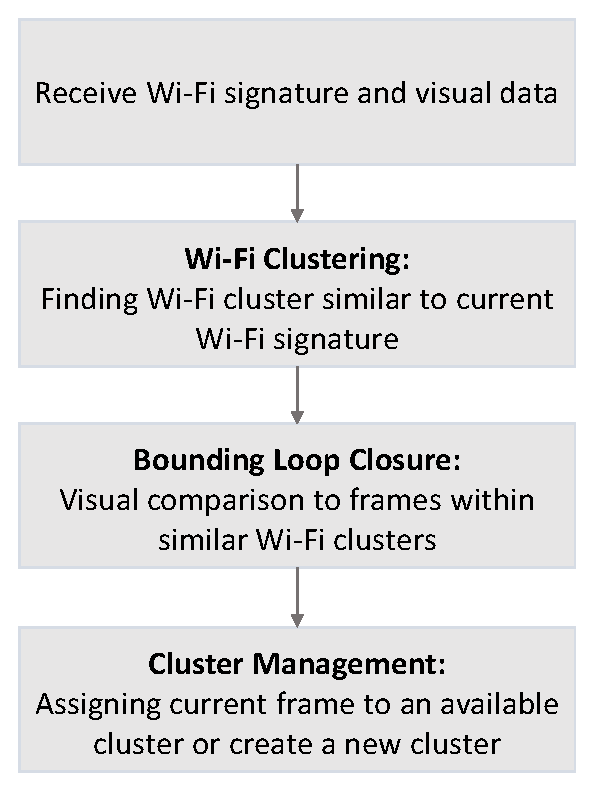
\includegraphics[width=0.3\textwidth]{Figure2_a.eps}
	\caption{General approach to incorporate Wi-Fi into any visual SLAM algorithm.}
%\vspace{-20pt}
\label{fig:gen_approach}
\end{figure}
\begin{figure}
	\centering
	\includegraphics[width=0.3\textwidth]{Figure2_b.eps}
	\caption{Visual representation of Wi-Fi clusters created on one dataset.}
%\vspace{-20pt}
\label{fig:cluster_rep}
\end{figure}

%\begin{itemize}
\textbf{Wi-Fi and Visual Association:} The first step is to associate a visual frame (image) with a corresponding Wi-Fi signature. For every 3 or 4 meters, the robot or mobile device pauses for about 10 seconds for Wi-Fi signature aggregation. Then, it associates any visual frame that follows with this Wi-Fi signature until the next pause.\\
\textbf{Wi-Fi Clustering:} Each Wi-Fi cluster represents a spatially separate region in the environment and has a representative Wi-Fi signature. 
It includes those frames which their signatures are similar to the representative signature and have at least one visual edge to another frame within the same cluster. \zaki{A visual edge represents a visual transformation between correspondent visual frames calculated through alignment of their keypoints.} In this module, we compute the cosine similarity between the Wi-Fi signature of the current frame and the representative signatures of all available Wi-Fi clusters within the database to find {similar clusters}. Any cluster within a threshold level of similarity is considered similar. These {similar clusters} represent spatial proximity to the current frame.\zaki{Figure~\ref{fig:cluster_rep} shows a visual representation of clusters created in one of our datasets.}\\
\textbf{Bounding Loop Closure Search:} A major challenge in SLAM is the problem of identifying a previously visited place. For example, if we go in a loop along the corridors of a building, we need to be able to recognize that we are back at the starting point once we complete the loop. This problem is called {\it Loop Closure}. As the map grows, SLAM algorithms accumulate many frames and it becomes computationally intensive to check for loop closures. Reducing the search space greatly benefits the timely working of a SLAM system. In this module, we reduce the search space by comparing the current frame only to frames within {similar clusters}. We do this to emulate comparison to frames from close-by regions.\\
\textbf{Cluster Management:} After permissible visual comparisons, the next step is to assign the current frame to the "correct" cluster. If any visual edge is added between the current frame and any frame within {similar clusters}, the current frame is assigned to that cluster. If there are multiple such clusters, the one with the highest cosine similarity is chosen. If no valid visual edges or {similar clusters} are found, a new Wi-Fi cluster is created and the Wi-Fi signature of the current frame is assigned as the representative signature of that cluster.

\zaki{In the beginning and upon receiving the first visual frame and Wi-Fi signature, we create the first cluster and assign the Wi-Fi data as its representative Wi-Fi signature. When a new visual frame along with its correspondent Wi-Fi data is received, we compute the cosine similarity between its Wi-Fi signature and the representative Wi-Fi signatures of all available clusters in the \it{Wi-Fi Clustering} module to find similar clusters. Similar clusters are the one which their cosine similarity is higher than a certain threshold. In the next step in \it{Bounding Loop Closure Search}, the new visual frame is compared against the visual frames within similar clusters to find acceptable visual transformations. If a visual transformation is accepted between the current frame and any frame within one of similar clusters, the current frame will be assigned to that cluster. Upon having more than one such clusters, the one with highest Wi-Fi similarity is selected. If no such visual transformation is available, a new cluster will be created and the current Wi-Fi signature would be assigned as its representative Wi-Fi signature. This process is executed for all frames.}
